\section{Stakeholders}
In het vooronderzoek wordt er een stakeholdersanalyse gemaakt om de stakeholders in beeld te krijgen.
De stakeholders zijn individuen of organisaties die invloed of belang hebben bij het project.
De product owner zal de mogelijke markt van kleine klanten representeren.
Dit wordt gedaan omdat Snakeware niet kleine klanten heeft die gebruikt kunnen worden als stakeholders.
% Sommige externe stakeholders zullen gerepresenteerd worden door een gekwalificeerde interne medewerker van Snakeware.
% Dit wordt gedaan omdat de afstudeeropdracht een proof of concept is, en de klanten van Snakeware hier nog niet bij betrokken worden.
Als na de afstudeerperiode het een succes blijkt te zijn en Snakeware wilt het verder ontwikkelen dan wordt contact opgezocht met de externe stakeholders (potentieele kleinere klanten). 
Verder is er een invloed matrix gemaakt (figuur \ref{fig:StakeholdersInvloedMatrix}) om de invloed en belang van de stakeholders te visualiseren. \\
Het project bestaat uit de volgende stakeholders:
\whitespace
\textbf{Product Owner:}
De Product Owner is verantwoordelijk voor het vertegenwoordigen van de belangen, eisen en wensen van de kleinere klanten.
Deze kleinere klanten worden niet als individuele stakeholders beschouwd, aangezien Snakeware geen afzonderlijke kleine klanten heeft.
Om deze reden wordt er binnen Snakeware een gekwalificeerde persoon ingezet om hen te vertegenwoordigen.
\whitespace
\textbf{Afdeling R\&D:} De afdeling R\&D van Snakeware zijn de ontwikkelaars van het huidige \gls{CMS} en kunnen veel inzicht bieden in de huidige situatie / problemen.
\whitespace
Het product bestaat uit twee software-applicaties een frontend die de data weergeeft aan de gebruiker, en een \gls{CMS}-API die de data serveerd voor de frontend.
Deze twee software-applicaties worden na de afstudeerperiode overgedragen aan twee verschillende diseplines in Snakeware, namelijk de backend en frontend developers.
\\
\textbf{Backend developers:} De \gls{CMS}-API wordt aan het einde van de afstudeeropdracht overgedragen aan de backend developers van Snakeware.
Tijdens de ontwerp en realisatie fase kan er voor advies gevraagd worden over hoe de \gls{CMS}-API het best ontworpen / gerealiseerd kan worden. \\
\textbf{Frontend developers} : De interface applicatie die gemaakt wordt om de data te tonen aan de gebruiker wordt ook overgedragen aan het einde van de afstudeeropdracht.
Tijdens de ontwerp en realisatie fase kan er voor advies gevraagd worden over hoe de inteface het best ontworpen / gerealiseerd kan worden.
\begin{graphic}
    \captionsetup{type=figure}
    \caption{Stakeholders invloed matrix}
    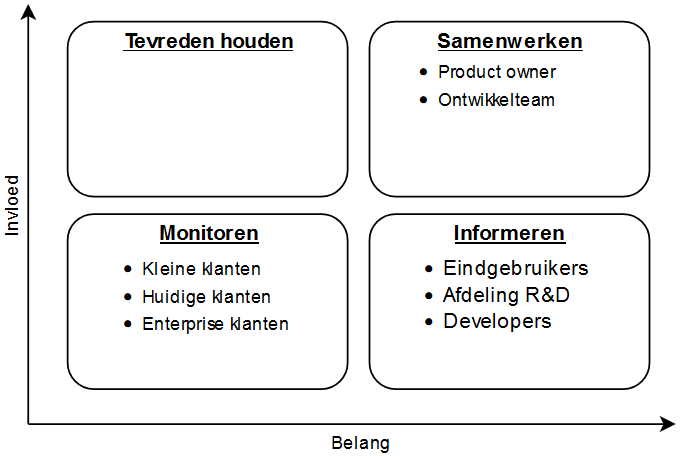
\includegraphics[scale=0.4]{StakeholdersInvloedMatrix}
    \label{fig:StakeholdersInvloedMatrix}
\end{graphic}

